
\begin{textbox}{Key concepts I}
\red{Bag-of-words (BOW)}

\green{\emph{type} vs. \emph{token}}
\emph{To be or not to be.} = 6 \emph{tokens}, 4 \emph{types}.

\red{\emph{type}} descriptive criterion\footcite[cf.][12]{stroustrup}

\red{\emph{token}} unit of analysis\footcites[cf.][12]{stroustrup,attentionMerchants}


\bigskip

\underline{Key topics}
\begin{itemize}
    \item One
    \item Two
    \item Three
\end{itemize}

\end{textbox}









%--------------------------------------------------------------
\section{Tools}



\begin{textbox}{Lorem Ipsum}
test  \sep test \sep test \sep test

\bigskip

\green{Visualize}
\begin{enumerate}
\item \textbf{present} your data
\item \textbf{analyze} the information
\item \textbf{explore} the findings
\end{enumerate}

\end{textbox}


\begin{textbox}{Voyant Tools}
 \href{https://voyant-tools.org/}{Voyant Tools} \sep \href{https://voyant-tools.org/}{Voyant Tools}

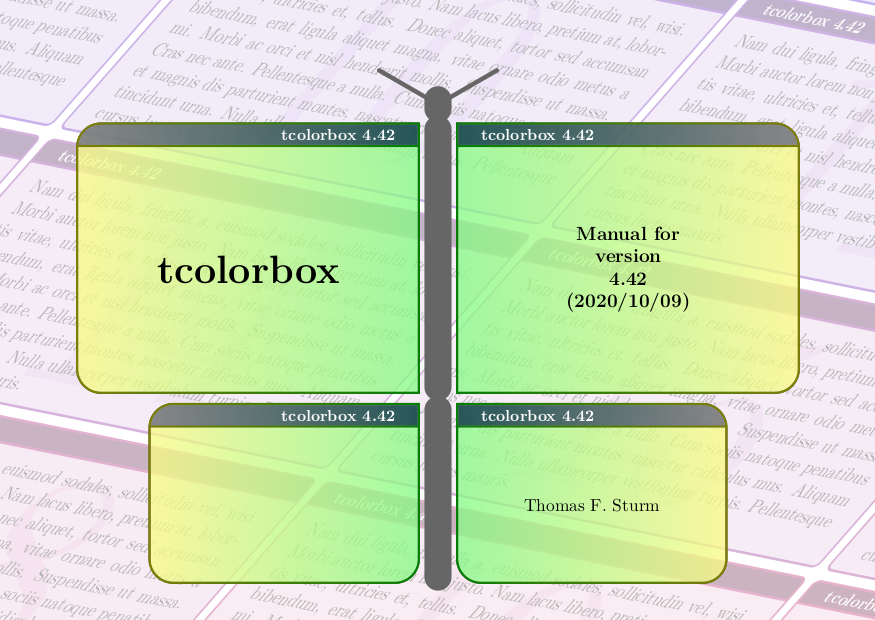
\includegraphics[width=\textwidth]{img/example-image.png}
\end{textbox}




\begin{textbox}{Project Gutenberg Texts}
\begin{tabular}{r|p{0.8\textwidth}}\scriptsize
    84 & \href{http://www.gutenberg.org/ebooks/84}{Frankenstein; Or, The Modern Prometheus by Mary Wollstonecraft Shelley} \\
    6087 & \href{https://www.gutenberg.org/ebooks/6087}{The Vampyre; a Tale by John William Polidori} \\
    696 & \href{https://www.gutenberg.org/ebooks/696}{The Castle of Otranto by Horace Walpole} \\
    42 & \href{https://www.gutenberg.org/ebooks/42}{The Strange Case of Dr. Jekyll and Mr. Hyde by Robert Louis Stevenson}
\end{tabular}

\end{textbox}





\begin{textbox}{Key concepts}
\red{Bag-of-words (BOW)}


\green{\emph{Zipf's Law}}

\mycommand{_&§!$§/()$}{code}
\mycommand{shutdown -h now}{to shutdown}

\end{textbox}


%--------------------------------------------------------------
\section{Programming}

\subsection{Code boxes}


% first argument: minted programming language name, for example.. css, c, cpp, etc.
\begin{codebox}{r}{Code box using R}
# Install
install.packages("tm")  # for text mining

# Load
library("tm")

# text <- readLines(file.choose())
# Read the text file from internet
filePath <- "http://www.internet.com/text.txt"
text <- readLines(filePath)

\end{codebox}


% first argument: minted programming language name, for example.. css, c, cpp, etc.
\begin{codebox}{cpp}{Code box using C++}
for (auto element : vector) 
{
    sum += element;
}
\end{codebox}

\section{Graphics}
The following is an example for a custom graphics command

\mygraphics{img/example-image.png}



\section{Other types of boxes}

\begin{alerttextbox}{The Alert Block}
\lipsum[10]
\end{alerttextbox}

\begin{myexampleblock}{The Example Block}
\lipsum[22]
\end{myexampleblock}

\mycommand{https://github.com}{Github Link Example}

\begin{myblock}{Branch}
Explanation
\end{myblock}

\begin{myblock}{Commit}
What's a commit?
\end{myblock}


\begin{myblock}{Staging}
s. Index
\end{myblock}


\begin{myblock}{Lipsum}
\lipsum[55]
\end{myblock}

\begin{textbox}{Yay Quotes}

\begin{quote}
    Yay, a quote!
\end{quote}

\begin{quote}
    Yay, a longer quote! \lipsum[5]
\end{quote}
\end{textbox}